\newcommand{\aipspp}{{AIPS++}}

\section{Introduction} 

\noindent
This document outlines the requirements for Very Long Baseline
interferometry (VLBI) to enable data from the world's major arrays
(EVN, VLBA, APT, CMVA, JNET) to be reduced within \aipspp. The primary
instrument models for software development in \aipspp\ have been
connected--element (CE) arrays like the VLA, WSRT and ATCA, although
much care has been taken to adopt a formalism that is not tied to any
specific instrument or type of data (the Measurement Equation). There
are, however, specific requirements for (VLBI) that should be
identified and incorporated into the software development at an early
stage, including special measures to allow for astrometric and
geodetic VLBI data processing as well as Space VLBI. The purpose of
this document is to outline those requirements. No attempt has been
made to separate the specific VLBI requirements from those that are
already defined for other interferometer data processing. However, it
is clear that the requirements for VLBI presented in this document
do not form a complete set of functionality either; for many
detailed and non VLBI specific functions we have assumed that the
equivalent of AIPS tasks will be available. We think it is understood
that these things will be required if \aipspp\ is to replace AIPS
eventually.

In discussing VLBI-specific requirements, parallels to existing or
developing AIPS routines will be drawn. Of course, some fraction of the
requested functionality is not available in AIPS, although in some
cases (notably for Space VLBI) it is under construction. 

The final list of possibly interesting functions for \aipspp\ has
become quite lengthy. It is clear that some of these tasks will not
emerge without specific effort from the interested parties, but we
feel it is important to list all of them, in order to prevent that the
future implementation of some of these is made difficult (or
impossible) in design decisions.

This document has been produced after discussion with NRAO, EVN, JIVE
and ATNF staff, and draws on previous documents such as \aipspp\ Note
185, various \aipspp\ Consortium User Specifications, a draft document
by Tony Beasley (NRAO) on VLBI requirements, and a draft of
Post-Correlation Data Processing Requirements for the Enhanced EVN by
Dave Shone (Jodrell Bank). A draft version was discussed at a Workshop
on VLBI Requirements for \aipspp\ held in Alcala de Henares (Spain) on
22 October 1996. Participants included, besides most of the authors,
Francisco Colomer, Carla Fanti, Mike Garrett, Leonid Gurvits, Kari
Lepp\"anen, Maria Massi, Jan Noordam, Richard Strom and Peter
Wilkinson.

Our approach is to follow the data path from correlator to image (or
other final product) in \aipspp\ (Figure \ref{flow}), and point out
the specific VLBI requirements, including those for Space VLBI, 
along the way. 

\section{General Considerations}

\subsection{Programmability}

Most of this document deals with required functionality of \aipspp\ 
``tasks''. However, the VLBI community is also very concerned about
the programmability of the package. Traditionally, many VLBI
astronomers have (necessarily) been involved in algorithm development.
And it is clear that this is a continuing effort in all aspects and
stages of VLBI processing. It is recognized that classic AIPS has
imposed a high threshold for non--specialists to test and implement
new methods.

In \aipspp\ there are many layers of increasingly complex software. It
is hoped that the user interface and script language (Glish) will
provide a platform for simple data operations and straightforward
processing. However, it seems unavoidable that at least some fraction
of algorithm implementation by VLBI astronomers requires the use of
compiled code. Because of the large datasets involved in VLBI
processing, speed is a consideration for these projects. Easy access
to class libraries, interfaces to C and FORTRAN, and documentation on
the appropriate level seem to be required to ensure programmability.
Skeleton tasks, tutorials and even training courses should be
considered.

\subsection{User Access to Data}

There need to be flexible and simple ways for the users to manipulate
their $u,\! v$ datasets, for example:

\begin{itemize}
  
\item The user should be capable of using the host system's
  capabilities and utilities to manage his\slash her datasets. The datasets
  should use a normal file name, and the user should be able to use
  the host directory hierarchy to best organize the data.

\item Tasks should generally take multiple input $u,\! v$ datasets where
  this makes sense. For example, the map making program should be
  capable of taking multiple input datasets, all of which contribute
  to the output images with user defined weights.
  
\item There needs to be a flexible way for the user to select the
  particular subset of data, in a dataset, to be processed. As well as
  selection based on time, antenna number, frequency, subarray, etc,
  it should be possible to select based on the values of other data
  (including monitor data).

\item It should be possible to extract a subset of data from a dataset
  and manipulate it in some powerful command language. This would
  include displaying the data and optionally replacing it in the
  dataset (e.g.\ multiply the amplitudes for some antenna by an
  arbitrary factor).

\item It should be possible to extract a subset of data from a dataset
  in a variety of formats (e.g.\ FITS or plain text) in order to
  transfer the data to other programs or packages. It should also be
  possible to read the modified data back into \aipspp\ using the same
  formats.

\item For applications where the built--in tasks and command language
  features are insufficient, there needs to be a program interface to
  allow the casual programmer reasonable access to the data. Some
  flexibility and efficiency can be sacrificed in making this
  interface comparatively simple.  FORTRAN programmers should be
  supported.

\end{itemize}


\subsection{Documentation}

Another point we want to emphasize is one of documentation for
non--specialist users. Our users often have no previous experience in
synthesis imaging and start directly with VLBI. They need a
cookbook--like introduction as well as tutorials.

\subsection{Portability}

For the VLBI user community it is of great importance that \aipspp\ is
portable to all systems that have significant support in the global
VLBI community. At the moment these are mostly UNIX systems; besides
Solaris and SunOS, especially DEC Alpha, HP/UX and Linux platforms are
popular around the VLBI world.

\subsection{Examples of VLBI Experiments}

To get a feel for the possible data types that VLBI processing has to
take into account, we list below possible VLBI observations for which 
\aipspp\ processing and\slash or application development should be possible.

The first part of this list concentrates on data types that we
consider part of (future) standard VLBI practice:

\begin{itemize} 

\item continuum observations in single or dual polarization

\item spectral line observations in single or dual polarization
  
\item observations in which polarization, frequency, and\slash or pointing
  centre may be rapidly switching in time.
  
\item simultaneous observations in multiple frequency bands (e.g.\ for
  observing multiple lines simultaneously or multi--frequency
  synthesis or S/X), with variable numbers of channels within each band

\item pulsar-gated data
  
\item mosaiced observations with several\slash many pointing centres
  (e.g.\ large line sources, gravitational lenses).  This must be
  supported at both the $u,\! v$ dataset and image dataset level
  
\item polarization data with unequal $uv$--sampling, where all four
  polarization parameters are not available simultaneously, as might
  occur for networks with inhomogeneous polarization sampling or
  time-switching of the recorded polarization
  
\item combination of data from different observations that have
  different (but overlapping) spectral sampling
  
\item time--series data of profiles and visibilities (e.g.\ pulsar
  data with bin number as a data axis)
  
\item multi--array datasets (e.g.\ MERLIN+EVN)
  
\item multiple correlations from multi--field centre observations,
  for which the calibration should be identical (e.g.\  gravitational
  lenses)

\end{itemize}

\noindent
More specialized dataset types which could be taken into
consideration in the design of \aipspp\ are:

\begin{itemize}

\item space VLBI observations

\item observations during which the source changes structure (e.g.\ SS433)

\item cluster--cluster data (e.g.\  WSRT--VLA multi--antenna VLBI)

\item burst sampling for mm--wavelength VLBI

\item triple correlation (including the case where one of the visibilities
has a different frequency)

\item combinations of the above (e.g.\ pulsar gated data in
  cluster--cluster mode)

\end{itemize}

\begin{figure}
     \begin{center}
     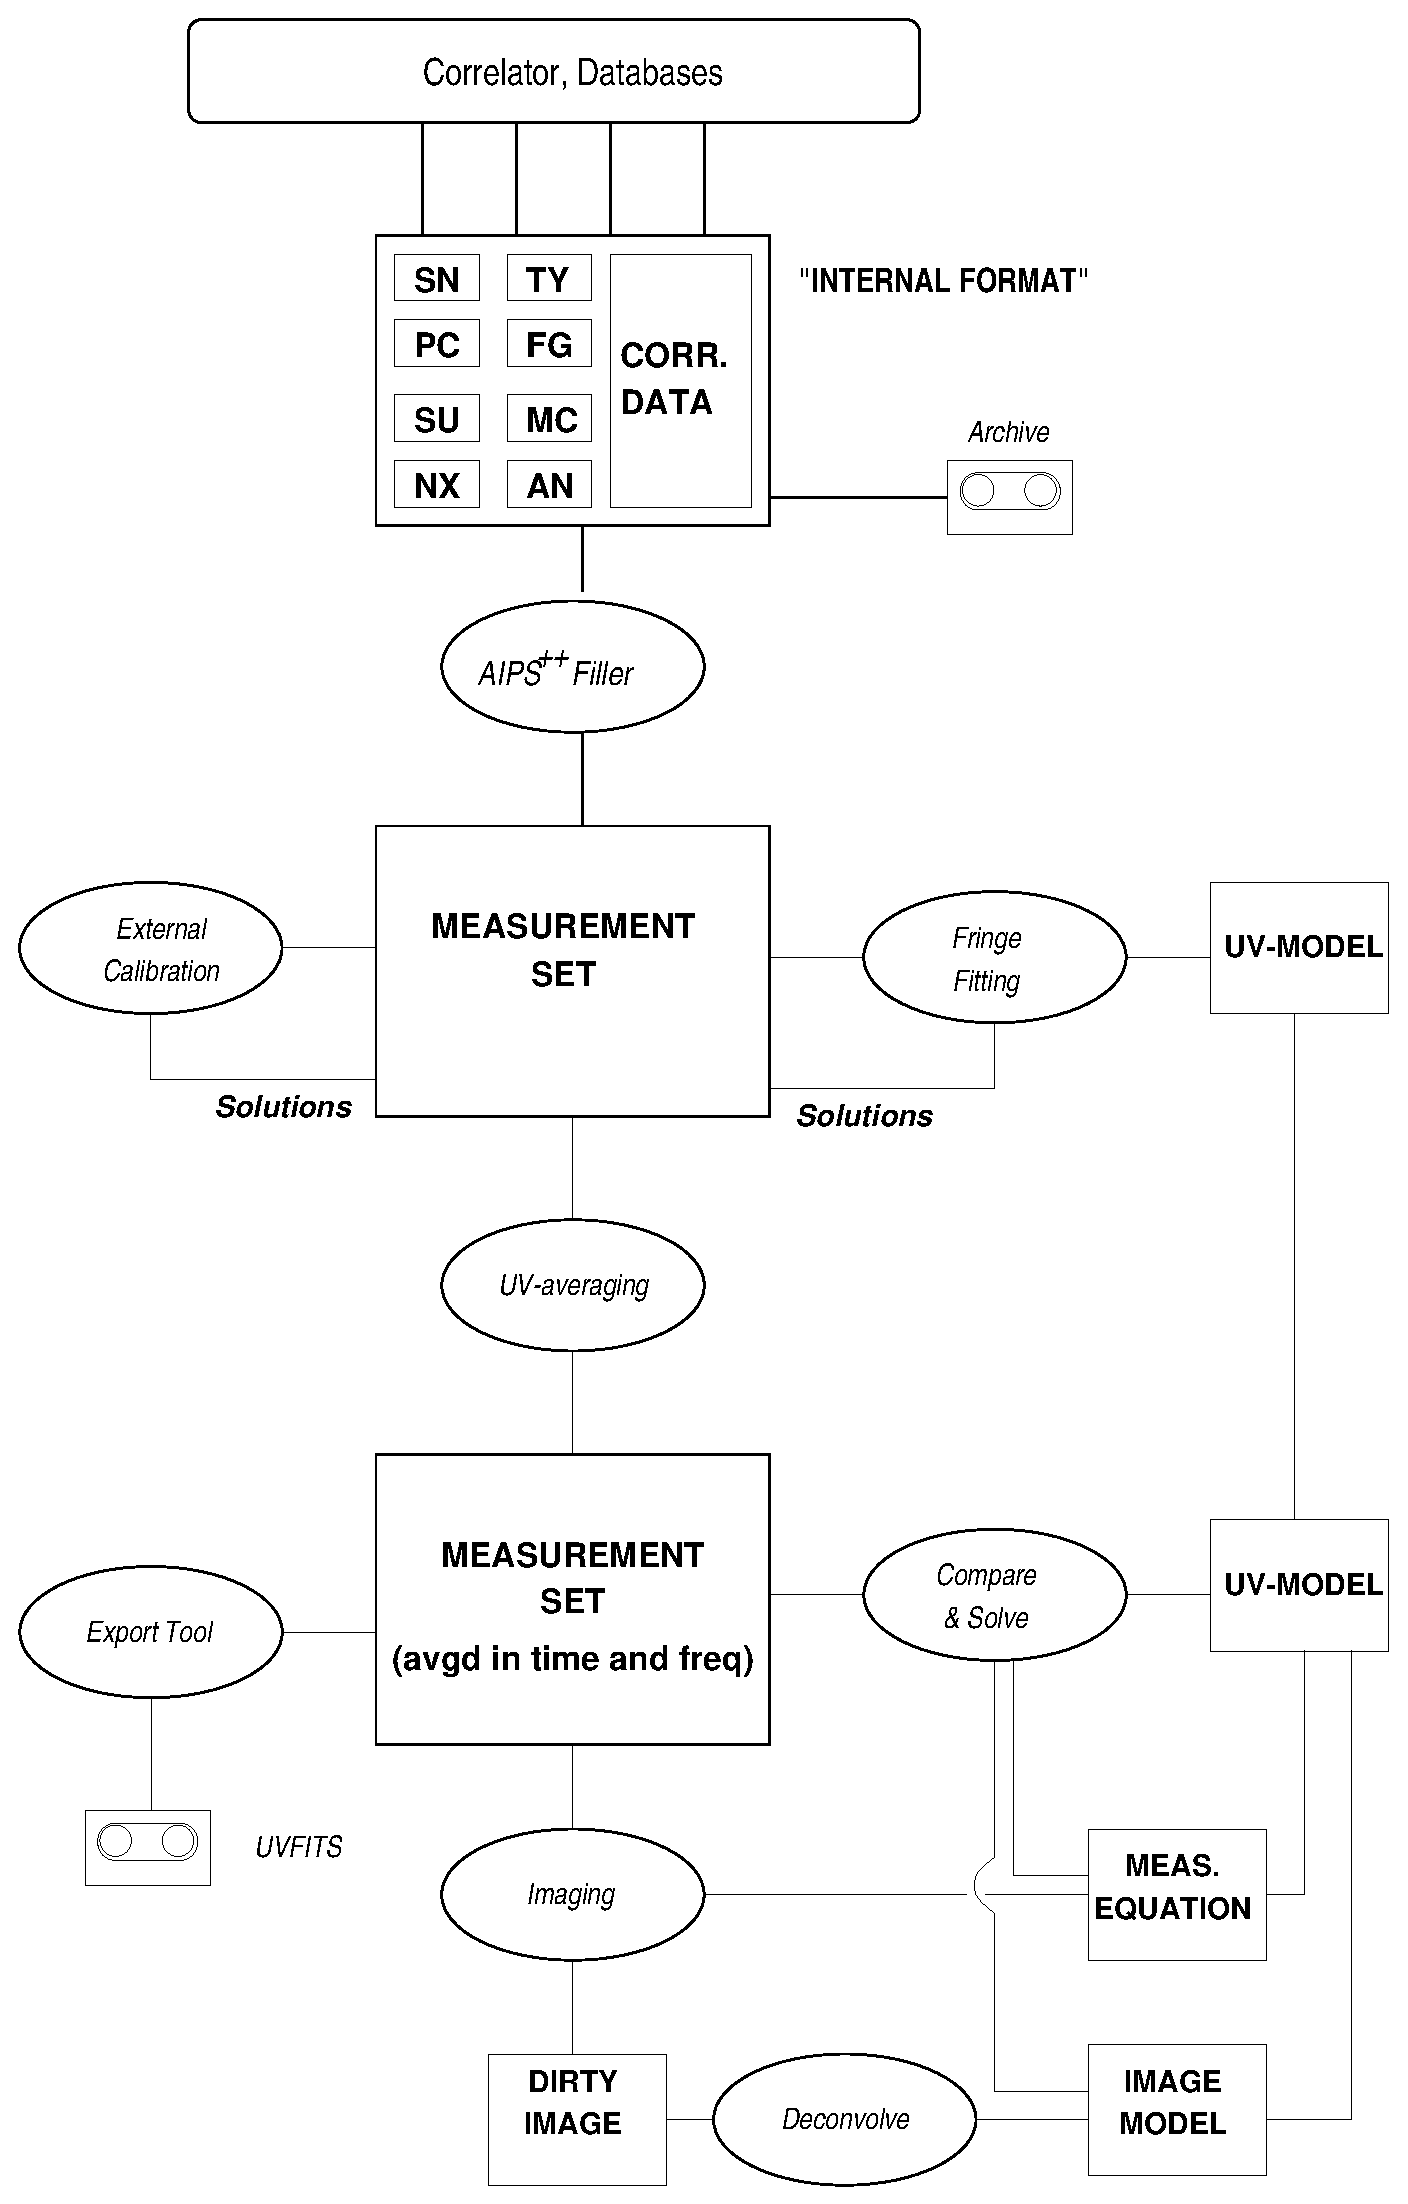
\epsfig{file=aipspp.ps,height=12.5cm} 
     \end{center}
     \caption[aipsflow]{\label{flow}\sl A possible model for data
       flow for VLBI data in \aipspp.  The correlator specific format
       may contain all the calibration data.  Examples of some of
       these are denoted in this figure by their classic AIPS table
       two letter codes: e.g.\ PC for phase cal data, SN for amplitude
       calibration for example based on state counts, TY for system
       temperatures, FG for flagging, MC for correlator model
       components. Standard reduction has a specific VLBI part which
       involves calibration based on external data and fringe fitting.
       This allows the Measurement Set to be averaged in frequency and
       time. Following this, standard imaging and (self)calibration
       techniques are available to improve the image quality and the
       model of the source and sky.}

\end{figure}

\section{Data--Loaders}

\subsection{Correlator Output}

We think that ideally data loaders for specific observatories and
correlators should not be required; data output from various places
should use a common format and data content to allow transparent
access by the users. The goal of the FITS standard is to establish
this. However, with the complexity of VLBI correlators and specific
requirements for calibration of certain observations, we fear that
such a wish is not realistic, and data loaders for the various
correlators (VLBA\slash MkIII\slash JIVE\slash SHEVE\slash K4) will be
required. Note that the Canadian S2 and Japanese VSOP correlators will
use the VLBA FITS binary table format. Furthermore, the JIVE
correlator also intends to use the FITS binary table format. For the
ATNF LBA this would be RPFITS (as in ATLOD), MkII correlators produce
UVFITS. However, FITS readers for VLBI are not only a matter of data
format, but in particular a matter of information content, providing
an instrument specific path to convert the data (content) to a data
set with extension tables suited for the calibration tasks. At least
all the required data loaders should be separate individual tasks, not
part of any generalized FITS readers (see section \ref{corerr}).  

It is part of the \aipspp\ consortium requirements that the code can
be used for on--line data reduction, e.g.\ at correlation time; this
requires that it will be possible to develop data loaders for internal
archive formats at various correlators. 

\aipspp\ must be aware of any additional data carried in MkIV, VLBA,
MkIII, S2 and VSOP format before correlation. Support, in this
context, may be no more than maintenance of an awareness of the
contents and structure of this data. In principle, these different
formats should not have any impact on post--correlation data formats;
in practice, we should be aware of additional data which are carried
in these or any new formats, since these may become relevant to some
aspects of off--line data--processing (e.g.\ the fixed phase offset
between upper and lower sidebands in MkIII and MkIV).

Some correlators (notably MkIII) are known to produce redundant data;
to obtain all baselines in a specific experiment multiple correlator
passes are necessary and sometimes data on certain baselines is
produced more than once. Data readers for such data should allow the
user to select a certain correlator pass or store redundant data
(see also section \ref{redata}). 

\subsection{Calibration of Correlator effects}
\label{corerr}

Individual correlators will introduce different digital signal
processing effects which will need to be corrected; one example of
this is the FFT artifact in VLBA data. State count corrections (if not
performed by the correlator) are another example.  Ideally we think it
is the responsibility of the correlators to deliver data in which such
specific calibration has been applied.  However, the AIPS approach for
VLBA data has been to apply this correction on input, by means of the
data loader (FITLD). Separate tasks for each correlator, each of which
potentially requires correction templates or additional information,
will be needed. (AIPS equiv: ACCOR, sections of FITLD).

\subsection{Auxiliary data}
\label{auxin}

Similar to CE interferometers, VLBI uses a large number of associated
data sets for calibration and data flagging. VLBI is different in the
sense that this information is not always available\slash applied during
correlation and needs to be appended to the data product. Below we
list a number of such data sets that possibly need to be read from
external sources. Because it can not be anticipated beforehand which
calibration method will be used for a certain project (e.g.\ which 
ionospheric model), this requires in some sense that the Measurement
Set can be flexibly extended.

\noindent Examples are:
\begin{itemize}
  
\item meteorological data (e.g.\ for tropospheric correction)

\item GPS timing data

\item phase calibration data based on pulse cal detection at telescope
  or correlator

\item amplitude calibration based on state count statistics

\item ionospheric data of various sources (e.g.\ TEC monitoring)
  
\item accurate total power measurements to monitor phase excursions
  for mm VLBI
  
\item specific data associated with record and playback processes
   
\item for Space VLBI additional information will be carried along with
  the data (e.g.\ satellite parallactic angle, sensitivity, orbit,
  downlink information, ``delta--t'' tables etc.), and tasks to read,
  process and apply corrections based on these data will be required

\end{itemize}

\section{Data structure}

\subsection{General Requirements}

First we list the some general data system requirements. These are
probably already included in the infrastructure development for CE data in
\aipspp\ and required for VLBI.

\begin{itemize}
  
\item the data system file format(s) should be accessible from all
  supported machines without conversion
  
\item simultaneous sub--netting should be supported
  
\item coordinate handling must be very general and allow different
  coordinate systems and ephemeris information to be carried along
  
\item support for data with non--regular increments in coordinate axes
  is required (e.g.\ non linear velocity axis)
    
\item near field imaging should be supported

\item it will be necessary to merge data sets
  
\item support for data errors should be fundamental to the data
  system, providing a basis for support of data error handling in a
  variety of applications:

  \begin{itemize}

  \item easy generation of error models

  \item error propagation through a series of tasks

  \item error images associated with astronomical images
    
  \item plotting error bars on spectra and profiles

  \item automatic warning if contour levels are below noise

  \item error--based blanking in display of results

  \item properly formatted errors when data are extracted for tabulation

  \end{itemize}
  
\item a processing history should be maintained for each data set that
  can be reviewed by the astronomer, using an easy to use
  browser, which allows sorting and editing
    
\item the user should have access to both data values and the
    ``header'' values that govern the interpretation of the data.

\end{itemize}

\subsection{Quantities}

All quantities such as antenna position, sky position, time, earth
orientation parameters, delay and rate should have sufficient
precision for VLBI purposes (including Space VLBI), requiring a double
in most cases.  There should also be ID strings attached to them to
specify the coordinate system they refer to. It will be insufficient,
for example, to demand that all \aipspp\ antenna positions will be
IERS XYZs. The VLBA uses USNO terrestrial\slash celestial frames and EOPs,
while the JIVE correlator is likely to use IERS frames. These
differences are important for VLBI observing, particularly for
astrometric\slash geodetic experiments.

For Space VLBI it is necessary that \aipspp\ supports the motion of an
orbiting antenna.

It would be advantageous (and possibly required for use at some
correlators) that \aipspp\ allows data to be stored in the lag domain.

\subsection{Version Typing}

All programs should enter and\slash or pass complete version information
concerning any (correlation) model applied to the data (e.g.\ 
geometric, tropospheric\slash ionospheric, source structure) to enable
complete reconstruction of the total delays measured. Ideally, it
should be possible to update a specific component in the model (e.g.\ 
take out and replace the geometrical model).

\subsection{Multi-File Datasets}

The short integration times and abundant channelization required for
VLBI data (due to weak phase stability) leads to large datasets,
particularly for spectral-line experiments. The ability to
transparently address large datasets spread across many disks or tapes
is of growing importance for VLBI data reduction, and should be
implemented in \aipspp.

The data system should support the merging of correlation data and
calibration data from different correlators.

\subsection{Inhomogeneous Arrays}

In the calibration (and imaging) steps it should be possible to treat
inhomogeneous arrays in which not only antenna characteristics vary
widely (e.g.\ antenna size, system temperature), but also feed
specifications are quite different (e.g.\ linear or circular feeds and
equatorial or alt--azimuth mounts). Moreover, calibration procedures
can differ between different telescopes (e.g.\ single dish vs.\ phased
arrays).

\subsection{Variable Integration Times}

In the case of space VLBI or wide field imaging, the ability to have
different integration times on different baselines will be needed.
This should be possible in the \aipspp\ table system.

\subsection{Redundant Data}
\label{redata}

Some correlators produce redundant data when particular baselines are
correlated more than once. Robust handling of these cases is desired.
Some users will choose to resolve these redundancies at the data
loading stage, but there are many advantages to allow these
redundancies to be incorporated in the data structure and to be
resolved during processing. This would also allow \aipspp\ to be used
at these correlators to manage their data products.


\section{Calibration}

\subsection{General Comments}

We start with a list of features that the VLBI community thinks are 
useful for calibration strategies in general:

\begin{itemize}
  
\item Calibration, like flagging, should be reversible, with the
  ability to store calibration information and apply it
  ``on--the--fly''. However, it should also be possible to apply
  the derived calibration in order to create a new,
  calibrated data--set.
  
\item Calibration should be made as generic as possible; site
  specific\slash instru\-ment dependent code should be kept to a
  minimum.
  
\item Calibration of data should be possible from derived tables of
  instrumental parameters such as system temperature and gain vs.\
  elevation. It should be possible to derive such tables from
  calibration observations (e.g.\ derive gain--elevation tables).
  
\item The calibration process should include flexible interpolation
  and averaging of calibration data under the control of the user.
  
\item Redundancy (including $u,\! v$ crossing points) should be used
  whenever possible, as an additional constraint on calibration and
  self--calibration.
  
\item Cross--calibration of different instruments should be possible,
  (e.g.\  flux density scale, pointing) particularly where data from
  different arrays are to be combined.

\end{itemize}

\subsection{Amplitude Calibration}

Amplitude calibration of VLBI data is generally accomplished using
measured data from all the antennas, typically system or antenna
temperatures, sensitivity estimates (Jy\slash K), opacity corrections based
on tipping runs and CE estimates of source flux densities (e.g.\ the
phased VLA). There exist at least two fundamental log formats
containing this data (e.g.\ MKIII\slash MKIV and VLBA). Amplitude
calibration tasks capable of processing one or more of these external
input formats will be required. (AIPS equiv: ANCAL, ANTAB\slash APCAL).

In many spectral line VLBI projects amplitude calibration can be
derived by applying the system temperature and gain for a single
element in the network, and comparing the autocorrelation spectra on
all elements (AIPS equiv: ACFIT).

\subsection{Spectral Response}

Not only for spectral line purposes, but also for high dynamic range
continuum VLBI, it is necessary to calibrate the (complex) spectral
response for separate BBC channels of each telescope. In some cases
one has to rely on autocorrelation data to obtain the amplitude filter
shape. In other cases one can solve for phase and amplitude with
respect to the average amplitude and phase on each baseline, or derive
the bandpass by comparing to a source model (point source, model
components or map) (AIPS equiv: BPASS) or by fitting Chebysev
polynomials (AIPS equiv: CPASS).

Line VLBI is traditionally done with fixed frequency settings. To do
the Doppler tracking, necessary to get optimal spectral sensitivity,
resolution and correct labeling, one must shift each cross--spectrum
according to an accurate model of the antenna motions and the earth
geometry. This task also requires knowledge about the correlator model
that was used to take the data. It is required that the user can run
this task (AIPS equiv: CVEL) in \aipspp\ without the necessity to
supply detailed information about the observing conditions.

Spectral line VLBI requires the ability to change the spectral
sampling both by simple averaging, as well as by Fourier filtering.
Cases where this is needed are for example efficient fringe fitting,
optimal detection by matching line width, or combining data with
different spectral sampling. It is hoped that \aipspp\ will store
information about spectral resolution as well as the spectral
sampling.

\subsection{External Delay \& Phase Calibration} 

Most VLBI antennas inject tones into the signal path which are
extracted downstream to assess the varying electronic delays between
IFs. Routines to read, process and apply these corrections to data are
needed (AIPS equiv: PCLOD, PCCOR).

Information such as weather information, total-electron content
measurements, WVR data, CALC\slash SOLV output etc.\ may be available in
many cases. There is a need for tasks to read all these (section
\ref{auxin}). General tools will be needed to display, edit and
interpolate such data. Furthermore specialized tasks are required to
apply the corrections to the VLBI data.

Space VLBI may also require specialized external data.  For instance,
complicated phase corrections can be imagined to be necessary for
intrinsic satellite effects (e.g.\ delay flutter, frequency
variations). These can possibly be derived from external data; often
these will depend (in a complicated way) on the position of the
spacecraft.

\subsection{Fringe Fitting}

The weaker phase stability of VLBI data makes this the main area
requiring additional development compared to any \aipspp\ CE data
path. Robust and sensitive fringe fitting can in some cases be an
important factor for the detection threshold of VLBI. Fringe fitting
is a calibration task similar to other \aipspp\ calibration
requirements, but it is slightly more complex in that it requires the
data to be Fourier transformed to delay/rate. Further investigation
is required to determine how best to incorporate fringe fitting into the
Measurement Set formalism, with particular reference to the
separability of individual calibration factors.

As a minimum, the fringe fitting in \aipspp\ must have a similar
functionality as the combination of FRING and BLING in classic AIPS.
BLING offers a baseline--based fringe fit, FRING offers global fringe
fitting. The AIPS version has the capability to fit simultaneously for
single and multi--band delay or to treat all IF bands separately
(e.g.\ for ``manual phase cal''). This is required for fringe fitting
in \aipspp\ too, as well as the possibility to average different
Stokes data and to fringe fit in rate only for spectral line VLBI.

Fringe fitting should be robust in the absence of some of the IF bands
or in the case that some frequencies are flagged (e.g.\ due to
interference).  It should offer flexibility in setting the search
windows and report clearly about the computational resources requested
by the user.  Spectral averaging before delay searching is required in
order to allow large solution intervals for data sets with many
channels.  Different solution intervals for delay and rate could be a
useful option. It should be possible to display the data in the two
dimensional Fourier domain. In many cases the efficiency and
sensitivity of fringe fitting could be enhanced by (automatically)
limiting the search windows after an initial detection has been made.

Moreover, there are many enhancements requested over the functionality
of current AIPS fringe fitting. For detection of phase offsets between
hands of different polarization, fringe fitting of cross-hand data is
required. For polarization calibration it is also required that the
task retains carefully the phase difference between the two hands at
the reference antenna.

In order to take full advantage of the sensitivity of global fringe
fitting, it would be advantageous for the program to have a--priori
knowledge of the sensitivity of the fringe search.  With the source
model and basic knowledge of the elements involved in the network it
should be possible for the algorithm to pick a reference antenna and
work out the optimal way to acquire solutions for all elements. The
\aipspp\ task should allow control over which antenna is second in line
when the reference antenna fails to yield solutions. It should be easy
to determine the coherence time for individual baselines.

There is a need for implementing incoherent fringe fitting which is
used in millimeter VLBI. Fitting second order phase slopes
(acceleration) and other complex fringe-fitting routines will be
needed for Space VLBI. These include fringe prediction methods that
can be used to extrapolate fringe search windows forwards and
backwards in time and the possibility of phasing up the ground array
separately to improve sensitivity. To overcome the problem for many
spectral line projects of inaccurate knowledge of the spacecraft
position, a special fringe fitting routine could possibly be
anticipated which allows the derivation of the delay from a multi
component spectral line cube.

\subsection{Geodesy and Astrometry}

\aipspp\ must allow VLBI data to be subsequently
exported to geodetic or astrometric packages such as SPRINT and
CALC\slash SOLV. This requires full accountability of \aipspp\ in
order to derive ``totals'' from the correlator model and the result 
of fringe fitting. Data writers for these formats are required. (AIPS
equiv: CL2HF\slash HF2SV\slash HFPRT).  

For astrometric developments it must be possible to recalculate the
geometric model. It should be possible to replace part of the model
with different components (e.g.\ replace one tropospheric model with
another). It should be possible within the \aipspp\ environment to
derive antenna positions from interferometer data.

\section{Data Display and Editing}

The order of calibration, data display and editing is not fixed in
VLBI.  In many cases flagging is done within the self--cal and mapping
cycle, after a first fringe fit, but applying a--priori flags is often
the first thing done after data loading.

In the area of continuum data inspection a good model for
functionality is provided by the DIFMAP package. We hope that \aipspp\
can come up with a similarly  quick and intuitive way of inspecting and
editing data.

\subsection{$U,\! V$--data display}

In general VLBI has a strong demand for powerful tools to display the
data. Because of the large number of visibilities, each composed of
many IF bands and spectral channels, a lot of the time can be involved
in checking the data. A list of functionality that is expected in
this area is given below.

\begin{itemize}

\item display of data aggregated in various ways (e.g.\ averaged over
  a number of spectral channels). 
  
\item displaying amplitudes and phases baseline by baseline

\item displaying estimates of amplitude bias in amplitude plots

\item displaying both closure quantities: closure amplitude and phase
  
\item taking arbitrary cuts (e.g.\ circular, radial or a user--defined
  locus) through the $u,\! v$--plane interactively

\item setting windows in space and\slash or time interactively
  
\item expanding aggregates (e.g.\ clicking on an averaged
  multi--channel visibility to show the component spectrum).

\item plotting of spectra and correlation functions 
   (for different phase centers)

\item display of fringe rate spectra (AIPS equiv: FRPLT)
  
\item display of model data against observed data, for diagnostic
  purposes it should be possible to treat simulated data in a similar way

\end{itemize}

\subsection{Flagging Requirements}

Flagging will start with incorporating telescope based information
that is based on the log information. It is often augmented with
a--priori flags provided manually by the astronomer. In the calibration 
and imaging cycle, further flagging is performed.

\begin{itemize}

\item flagging should be reversible, with the ability to store
  flagging information and apply this on the fly
  
\item multiple level flagging to cater for different levels of
  severity of problems or different source of information
  
\item flagging on the basis of monitor\slash observing log data and
  tape motion
  
\item flagging from ``consistency check'' information, in particular
  redundancy, where possible, or crossing--points in the $u,\! v$--plane

\item flagging based on autocorrelation spectra
  
\item ``intelligent'' automated flagging for large datasets (e.g.\ 
  based on amplitude excursions, polarization)

\item baseline by baseline display and editing (including multiple,
  simultaneous baselines)

\item antenna based display and flagging (by interactively selecting
  baselines that involve a suspect antenna)

\item display of $T_{\rm sys}$, rate and delay data together with visibility
  data per interferometer
  
\item allow the display of flagged $u,\! v$ data in a different color
  along with the data and model

\end{itemize}
  

\section{Image Formation and Analysis}

The ability to process CE data implies that the \aipspp\ 
infrastructure development covers several aspects of VLBI processing.
Notably phase (only) and amplitude self--calibration routines,
coordinate handling, model--fitting, imaging algorithms will
become available because of these demands.

\subsection{Self--calibration and Imaging}

For VLBI processing it is important that (self--)calibration, data
inspection\slash editing, transformation and deconvolution are
integrated closely, as is available in DIFMAP.  When implementing such
features special care should be taken to warn (novice) users against
the dangers of making the ``data fit the model''.  It should be
possible to easily ``mix--and--match'' self--calibration,
transformation, and deconvolution tools, for example, using CLEAN to
deconvolve in the early stages, and NNLS or MEM later on when
CLEAN would begin to break--down. This also demonstrates the need to
make self--calibration use a generic model, which may be
CLEAN--components, an image, or a Gaussian model, or a combination.

More specific VLBI considerations are listed below:

\begin{itemize}

\item it should be possible to edit the list of clean components for self--cal

\item the possibility of using CLEAN polygons should be included

\item difference mapping should be supported
  
\item complex deconvolution is required to handle ``asymmetric''
  arrays (including telescopes with single polarization feeds)
  
\item fringe rate mapping (AIPS equiv: FRMAP)

\end{itemize}

\subsection{Image analysis and $U,\! V$ model fitting}

Although this strictly not an ``image analysis'' tasks, we note that
model fitting should be possible in both the image as well as
$u,\! v$--planes using point source, Gaussian or spherical models.  It
should be possible to use the resultant model in the same way as a
CLEAN component model in calibration and self--calibration. Specific
items are listed below:

\begin{itemize}
  
\item joint fitting for all four polarization parameters (as is done in
  the Brandeis package)
  
\item for Space VLBI it is required that model--fitting can cope with
  sparse $u,\! v$ coverage
  
\item it should be possible to display model data (i.e.\ from CLEAN
  components, fitting etc.) with observed and\slash or processed data
  simultaneously as well as data with model subtracted or divided

\item there should be tools available to do spectral line profile
  fitting, in order to derive velocities ands widths

\item in contour plots\slash grey scale plots, choose coordinate
  system when creating the plot file

\item possibly tools for gravitational lens transformation models
   
\item fitting of Zeeman profiles should be possible

\item it will be possible to develop tools to do proper motion analysis

  
\end{itemize}

In general we think that \aipspp\ should improve the capabilities to
produce publication quality figures from the data reduction package. 
For the VLBI community it important to be able to plot maps of sources
at different epochs or frequencies in a single figure.

\section{Conclusions}

We consider the prioritized list below the key to make \aipspp\ a
success in our community.

\begin{itemize}

\item programmability

\item development driven by scientific objectives

  \begin{itemize}
    
  \item Implement key functionality of existing packages with greater
    ease of use (as offered by DIFMAP for example)

  \item Offer applications that allow new science (e.g.\ polarization 
    processing)

  \end{itemize}

\item a complete path simple VLBI reduction, this involves:

  \begin{itemize}
  
  \item fringe fitting

  \item data loaders

  \item calibration tasks

  \end{itemize}

\end{itemize}

\noindent
We think that the work on fringe fitting should not be postponed too
long. This work is needed to verify that fringe fitting can be dealt
with in the current calibration formalism (the Measurement Equation).

There is considerable interest in the community to use the package in
an early stage even when only a small number of functions are
available, provided that are documented paths to transfer data from
\aipspp\ into AIPS and vice--versa.

%\end{document}
